\documentclass[
 %beamer-class options that do not change the layout can be added here
 UKenglish%,french%,ngerman(already default) ... %--- activate one (or more) language options as needed
 ]{beamer}%for detailed information see: texdoc beamer
\usetheme[%
 %noKITlogo, %--- activate to suppress the KIT logo on every standard slide
 %helvet, heros, %--- use one of these to have a fallback font as default
 %librefranklin %--- activate to have the fallback title font as default
 %cursor %--- activate to have the fallback typewriter font as default
 ]{KIT}

\graphicspath{{images/}}% this command from the graphics package allows to add folders (here subfolder "images") to be searched for graphic/image files
%\setbeamertemplate{navigation symbols}{}%--- activate to suppress the navigation symbols

%meta data fields: their content will be used for the title page (content of the optional arguments appear in parts in the footline)
 %(title and author will also be added automatically as PDF meta information)
\author[C.\, Knoesel]{Cedrico Knoesel}
\title[Multivariate Fine-Grained Complexity of LCS]{Multivariate Fine-Grained Complexity of Longest Common Subsequence}
\subtitle{By: Karl Bingmann \& Marvin Künnemann}
\institute[]{}
%\logo{\includegraphics[height=13mm]{beamericonarticle}}%e.g. insitute logo or project logo
                                          %(the beamericonarticle graphic comes from the beamer package
                                          % and must in case of need b replaced by your individual logo)
\titlegraphic{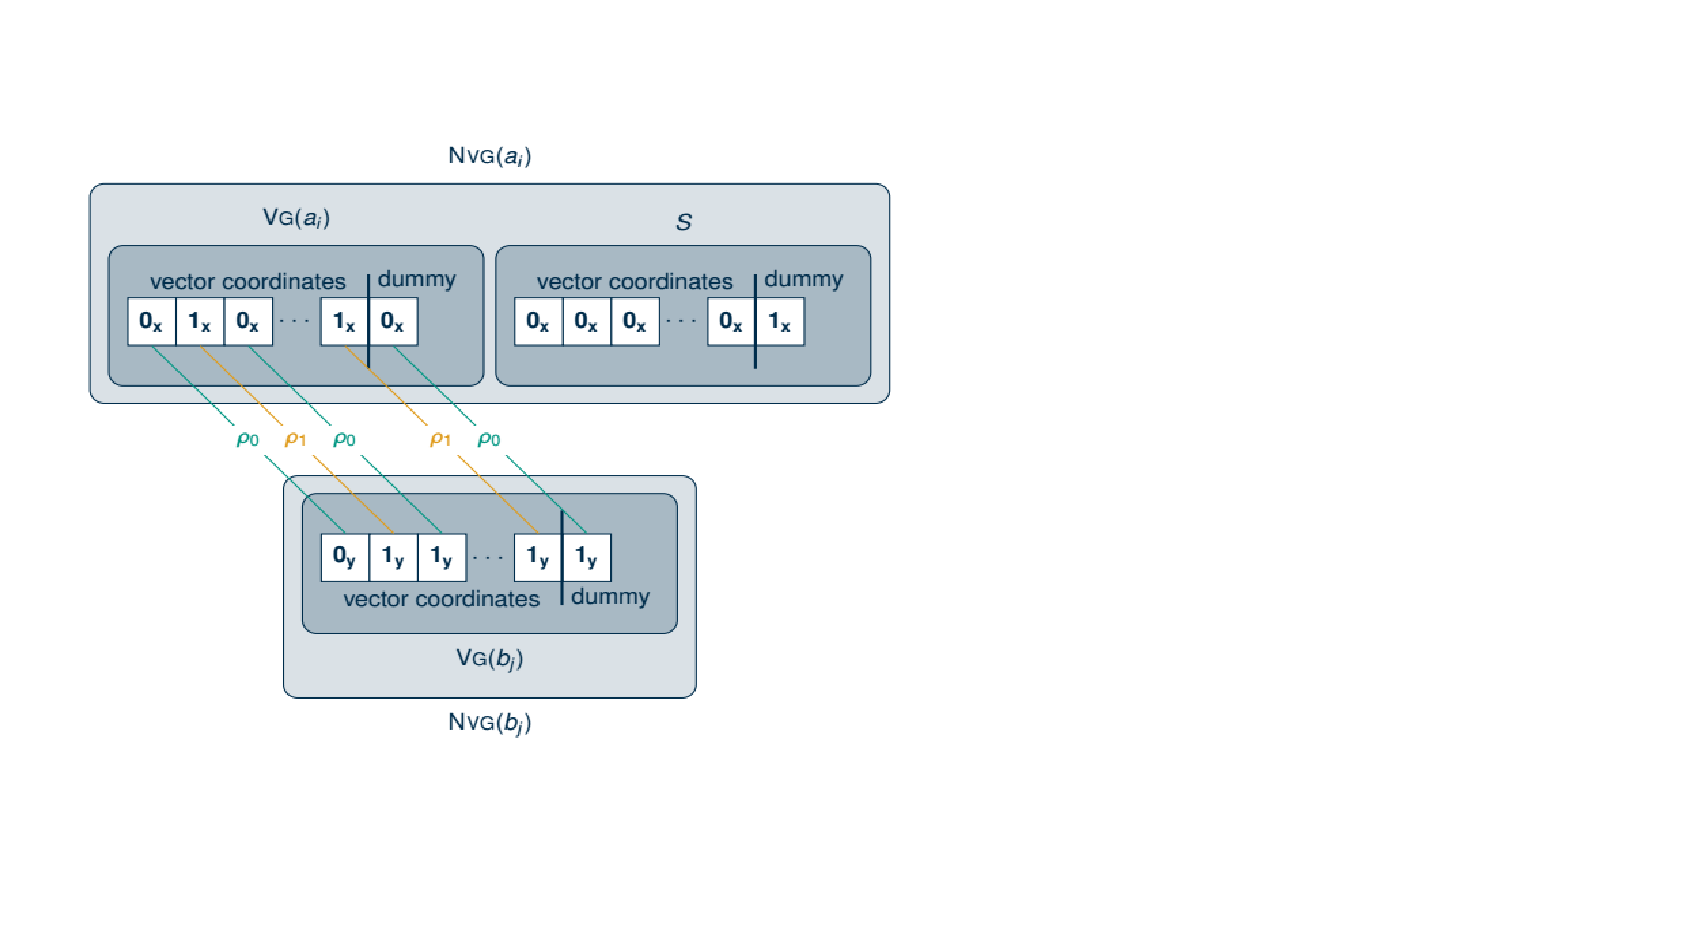
\includegraphics[height=\paperheight,trim=0 0 0 -9]{images/title-image-large.png}}%
%\date[\today]{} %--- activate to suppress date on title page




% Coordinate gadgets
\newcommand{\cgZeroX}{\mathbf{0_x}}
\newcommand{\cgOneX}{\mathbf{1_x}}
\newcommand{\cgZeroY}{\mathbf{0_y}}
\newcommand{\cgOneY}{\mathbf{1_y}}
\newcommand{\cg}[2]{\text{CG}(#1,#2)}


% Vector Gadges
\newcommand{\guardX}[1]{G_X(#1)}
\newcommand{\guardY}[1]{G_Y(#1)}
% example:
\newcommand{\exVGguardOne}[3]{\node[base, number, guard] (#3) at ($(#1) + (#2,0)$) {$1^{\gamma_2}$};}
\newcommand{\exVGguardZero}[3]{
		\node[base, number, guard] (#3) at ($(#1) + (#2,0)$) {$0^{\gamma_1}$};}
\newcommand{\exVGbigGuardZero}[3]{
		\node[base, number, big guard] (#3) at ($(#1) + (#2,0)$) {$0^{\gamma_3}$};}
\newcommand{\exVGendGuardY}[3]{
		\node[base, number, big guard] (#3) at ($(#1) + (#2,0)$) {$0^{n\gamma_4}$};}
		
		
\newcommand{\vg}[1]{VG(#1)}


% Normalised Vector Gadget
\newcommand{\nvg}[1]{\text{NVG}(#1)}

% TikZ für Graphiken in LaTeX
\usepackage{tikz}
\usetikzlibrary {arrows.meta}
\usetikzlibrary{calc}
\usetikzlibrary {graphs}
\usetikzlibrary {fit}
\usetikzlibrary {shapes}
\usetikzlibrary{shapes.arrows} 
\usetikzlibrary{shapes.geometric} 
\usetikzlibrary {calc} 
\usetikzlibrary{math} 
\usetikzlibrary {quotes} % for "label" on edges


% Paket zum Setzen von Algorithmen in Pseudocode mit kleinen Stilanpassungen
\usepackage[ruled,vlined,linesnumbered,norelsize]{algorithm2e}
\DontPrintSemicolon
\def\NlSty#1{\textnormal{\fontsize{8}{10}\selectfont{}#1}}
\SetKwSty{texttt}
\SetCommentSty{emph}
\def\listalgorithmcfname{List of Algorithms}
\def\algorithmautorefname{Algorithm}
\def\algorithmcflinename{Line}
\let\chapter=\section % repariert ein Problem mit algorithm2e


\usepackage{pgfplots}
\usepgfplotslibrary{external}
\tikzexternalize % Externalizes all tikz figures to PDFs
\tikzsetexternalprefix{build_tikz/} % Prefix of the directory on which all externalized figures are stored


\usepackage{subcaption}


\usepackage{siunitx} % for numbers and units
\usepackage{pifont}
\usepackage{marvosym}

\usepackage{blindtext}


\newlength{\nodeDistance}\setlength{\nodeDistance}{1.5cm} % default distance between two nodes
\newlength{\partitionRadius}\setlength{\partitionRadius}{0.4cm} % default radius of partition line

\tikzstyle{highlight} = [color=kit-red80]
\tikzstyle{dim} = [thin, color=kit-gray40]
\tikzstyle{tight} = [inner sep = 0.2ex]

\tikzstyle{node} = [draw,circle]
\tikzstyle{edge} = [draw, inner sep = 0.2ex]
\tikzstyle{cut edge} = []

\tikzstyle{color A} = [color=kit-orange100]
\tikzstyle{color B} = [color=kit-lightgreen100]
\tikzstyle{color C} = [color=kit-cyan100]
\tikzstyle{color D} = [color=kit-purple80]

\tikzstyle{partition} = [dashed, thick]
\tikzstyle{partition A} = [partition, color A]
\tikzstyle{partition B} = [partition, color B]
\tikzstyle{partition C} = [partition, color C]

% Ident algorithm2e code. Necessary because probably \parident is not defined
\setlength{\algomargin}{2ex}


% Using overlays in TikZ pictures.
% Inspired from https://tex.stackexchange.com/a/55849

% Keys to support piece-wise uncovering of elements in TikZ pictures:
% \node[visible on=<2->](foo){Foo}
% \node[visible on=<{2,4}>](bar){Bar}   % put braces around comma expressions
%
% Internally works by setting opacity=0 when invisible, which has the 
% adavantage (compared to \node<2->(foo){Foo} that the node is always there, hence
% always consumes space plus that coordinate (foo) is always available.
%
% The actual command that implements the invisibility can be overriden
% by altering the style invisible. For instance \tikzsset{invisible/.style={opacity=0.2}}
% would dim the "invisible" parts. Alternatively, the color might be set to white, if the
% output driver does not support transparencies (e.g., PS) 
%
\tikzset{
  invisible/.style={opacity=0},
  invisible text/.style={text opacity=0},
  %
  visible on/.style={alt={#1}{}{invisible}},
  text visible on/.style={alt={#1}{}{invisible text}},
  %
  alt/.code n args={3}{%
	\alt#1{\pgfkeysalso{#2}}{\pgfkeysalso{#3}} % \pgfkeysalso doesn't change the path
  },
}


\begin{document}

%several suggestions for the title page:
%\frame[empty]{\titlepage}

%\frame[empty,noKITlogo]{\titlepage}

%\frame[KITgreen]{\titlepage}

\frame[KITgreenhalf]{\titlepage}

%\frame[KITgreenhalfdarkblue]{\titlepage}

%\titlegraphic{\includegraphics[width=\paperwidth,height=0.55\paperheight,trim=0 0 -2 0]{beamericononline}}%
%\frame[KITgreenbottom]{\titlepage}

\begin{frame}[KITgreenTOC,t]{\fontsize{10}{10}\selectfont\textcolor{KITwhite}{Content}\hfill\lower2.5mm\hbox{\scalebox{0.72}{\KITlogo}}\kern3mm}
  \vspace*{-5mm}%
  \tableofcontents
\end{frame}


\section{Introduction}


\begin{frame}
	\frametitle{Find Parameter Relations}
	
	\begin{columns}[onlytextwidth]
	\column[t]{0.49\textwidth}
	\begin{tabular}{ll}
		\toprule
		\textbf{Relation} & \textbf{Restriction} \\
		\midrule
		$L \leq m \leq n$     &  \\
		$L \leq d \leq M$     &  \\
		$\Delta \leq n$       &  \\
		$\delta \leq m$       &  \\
		$\delta \leq \Delta$  &  \\
		\midrule
		$\delta = m - L$      &  \\
		$\Delta = n - L$      &  \\
		\midrule
		$d \leq Lm$               & \\
		$d \leq L^2 |\Sigma|$     & \\
		\alt<2->{\color{KITgreen}$\boxed{d \leq 2L(\Delta + 1)}$}{$d \leq 2L(\Delta + 1)$}   & \\
		$|\Sigma| \leq d$         & \\
		$\dfrac{L^2}{|\Sigma|} \leq M \leq 2Ln$ & \\
		\midrule
		$M \geq Lm/4$             & if $|\Sigma| = 2$ \\
		$M \geq nd/(5L)$          & if $|\Sigma| = 2$ \\
		\midrule
		$M \geq md/(80L)$         & if $|\Sigma| = 3$ \\
		\bottomrule
	\end{tabular}
	
	\column[t]{0.49\textwidth}
	Todo: Overview/Explanation of parameters
	\end{columns}

\end{frame}


\begin{frame}
	\frametitle{Find Parameter Relations}
	\framesubtitle{$d \leq 2L(\Delta + 1)$}
	
	\begin{theorem}
	For every LCS instance it holds that $d \leq 2L(\Delta + 1)$
	\end{theorem}

	\pause	
	
	\begin{proof}%
	\color{black}%
	\vspace{1ex}%
	\begin{columns}[onlytextwidth]
	\column[t]{0.01\textwidth}
	\column[t]{0.49\textwidth}
	Fix LCS $z$ of $x$ and $y$
	\begin{itemize}
		\color{black}
		\item<2-> Per definition $z$ obtainable by:
		\begin{itemize}
			\color{black}
			\item<2-> Deleting at most $\Delta$ positions from $x$ or
			\item<2-> Deleting at most $\delta$ positions from $y$
		\end{itemize}
		\item<3-> $x[1..i]$ contains $z[1..i-\Delta]$
		\item<3-> $y[1..j]$ contains $z[1..i-\delta]$
	\end{itemize}
	
	\vspace{2ex}
	\visible<4->{$\Rightarrow \min\{i-\Delta, j-\delta\} \leq L[i,j] \leq \min\{i,j\}$}
	
	\column[t]{0.49\textwidth}
	\visible<5->{
	Let $1 \leq k \leq L$
	
	\begin{itemize}
	\color{black}
		\item If $L[i,j] = k$:
		\begin{itemize}
			\color{black}
			\item<6-> $k \leq i \leq k + \Delta$ or
			\item<7-> $k \leq j \leq k + \delta$
		\end{itemize}
		\item<8-> For each $i' \in \{k, \ldots, k + \Delta\}$ and $j' \in \{k, \ldots, k + \delta\}$:
		\begin{itemize}
			\color{black}
			\item<9-> At most one $k$-dominant pair $(i',j)$ or $(i,j')$
		\end{itemize}
	\end{itemize}
	
	\visible<10->{
	$\Rightarrow |D_k| \leq \Delta + \delta + 2 \leq 2(\Delta + 1)$
	}
	
	\visible<11->{
	$\Rightarrow d \leq 2L(\Delta + 1)$
	}
	
	}
	
	\end{columns}
	\end{proof}
\end{frame}


\begin{frame}
	\frametitle{Find Parameter Relations}
	\framesubtitle{Overview}	
	
	\begin{columns}[onlytextwidth]
	\column[t]{0.3\textwidth}
	\KITpanel{1. Define Parameters}{%
		\begin{itemize}
			\item List parameters of problem $\mathbb{B}$
		\end{itemize}
	}{KITlightgreen}
	
	\column[t]{0.3\textwidth}
	\KITpanel{\color{KITwhite}2. Find Parameter Relations}{%
		\begin{itemize}
		\color{KITwhite}
			\item Bound parameters of $\mathbb{B}$
			\item Proof non-triviality of fully bounded parameter space
		\end{itemize}
	}{KITdarkblue}
	
	\column[t]{0.3\textwidth}
	\KITpanel{3. Find Reduction(s) from $\mathbb{A} \rightarrow \mathbb{B}$}{%
		\begin{itemize}
			\item Check reductions span full parameter space
			\item Derive lower bound for all parameter setting
		\end{itemize}
	}{KITiceblue}
	\end{columns}
\end{frame}


\begin{frame}
	\frametitle{Non-Triviality of Parameter Space}
	\framesubtitle{Definitions}

	\begin{definition}
	\end{definition}
\end{frame}

\subsubsection{Small LCS}
For the first reduction, we assume $\alpha_\delta = \alpha_m$, i.e., the number of deleted symbols in the smaller strings is asymptotically the same as the length of the smaller string.
This reduction is the same as used in a previous fine-grained analysis of \lcs{} \cite{Bringmann.2015}.




\begin{theorem}[Normalized Vector Gadget]
For any two vectors $a$ and $b$ of dimension $D$, there are two strings $\nvg{a}$ and $\nvg{b}$ with length $\bigO{D}$ such that
\[
L(\nvg{a}, \nvg{b}) = \begin{cases}
		\rho_0 & if \langle a, b \rangle = 0\\
		\rho_1 & otherwise
	\end{cases}
\]
for an appropriate $\rho_0 > \rho_1$.
\end{theorem}


\begin{theorem}
	For an OV instance $\mathcal{A} = \{a_1, \ldots, a_A\}$ and $\mathcal{B} = \{b_1, \ldots, b_B\}$ with $A \geq B$ and dimension $D$, we can construct the strings
\begin{align*}
	x &=& &\nvg{a_1}\ 0^\gamma\ \nvg{a_2}\ 0^\gamma\ \cdots\ 0^\gamma\ \nvg{a_A}\\
	y&=& 0^{A\gamma'}\ &\nvg{b_1}\ 0^{\gamma}\ \nvg{b_2}\ 0^\gamma\ \cdots\ 0^\gamma\ \nvg{b_B}\ 0^{A\gamma'}
\end{align*}

in time $\bigO{AD}$ with large enough $\gamma, \gamma' \geq |\nvg{a_i} + |\nvg{b_j}|$, satisfying:

\begin{enumerate}[(i)]
    \item $L(x,y) \geq \rho \Leftrightarrow \exists a_i, b_j:\; \langle a_i,b_j \rangle = 0$ \quad\quad (for some appropriate $\rho$)

    \item $|x|, |y| = \bigO{AD}$
\end{enumerate}
\end{theorem}	


\newcommand{\sLCSnvg}[3]{%
	\node[base, number, input, minimum width=4.5em, #3] (#1) at (base) {$\nvg{#2}$};
}
\newcommand{\sLCSnvgWithGuard}[4]{%
	\sLCSnvg{#1}{#2}{#4}
	\node[base, number, guard] (#3) at ($(#1.east)$) {$0^\gamma$};
}


\newcommand{\sLCSOr}{%
		\tikzstyle{base} = [minimum width=1.5em, inner sep=1pt, anchor=west]
		\tikzstyle{text element} = []
		\tikzstyle{number} = [minimum height=14pt]  
		\tikzstyle{guard} = [fill=lightgray]  
		\tikzstyle{guard edge} = [color=lightgray]
		\tikzstyle{big guard} = [fill=lightgray!75!black]
		\tikzstyle{big guard edge} = [color=lightgray!75!black]
		\tikzstyle{input} = [fill=cyan]
		\tikzstyle{input edge} = [color=cyan]
		\tikzstyle{cell} = [draw, minimum width=1.5em, fill=white]
		\tikzstyle{skipped} = [fill = lightgray!75!white]
		
		\node[base, text element] (eqX) at (0,0) {$=$};
		\node[base, text element, anchor=east] (x) at (eqX.west) {$x$};
		
		\coordinate (base) at ($(eqX.east) + (0.5,0)$);
		\sLCSnvgWithGuard{a1}{a_1}{a_g1}{skipped}
		
		\node[base, minimum width=3em] (a_dots_1) at (a_g1.east) {$\cdots$};
		
		
		\node[base, number, guard] (a_gj_left) at (a_dots_1.east) {$0^\gamma$};
		\coordinate (base) at (a_gj_left.east);
		\sLCSnvgWithGuard{aj}{a_j}{a_gj}{}
		
		\node[base, minimum width=3em] (a_dots_2) at (a_gj.east) {$\cdots$};		
		\node[base, number, guard] (a_gjB_left) at (a_dots_2.east) {$0^\gamma$};
		
		\coordinate (base) at (a_gjB_left.east);
		\sLCSnvgWithGuard{ajB}{a_{j+B-1}}{a_gjB}{}
		
		\node[base, minimum width=3em] (a_dots_3) at (a_gjB.east) {$\cdots$};
		
		\node[base, number, guard] (a_gA_left) at (a_dots_3.east) {$0^\gamma$};
		\coordinate (base) at (a_gA_left.east);
		\sLCSnvg{aA}{a_A}{skipped}
		
		
		\node[base, text element] (eqY) at (0,-1.2) {$=$};
		\node[base, text element, anchor=east] (y) at (eqY.west) {$y$};
		
		
		\coordinate (base) at ($(eqY.east) + (0.5,0)$);
		\node[base, number, guard, minimum width=3em] (b_left) at (base) {$0^{A\gamma'}$};
		\coordinate (base) at (b_left.east);
		\sLCSnvgWithGuard{b1}{b_1}{b_g1}{}
		\coordinate (base) at (b_g1.east);
		\node[base, number, input, minimum width=6em] (b2) at (base) {$\nvg{b_{2}}$};
		\node[base, number, guard] (b_g2) at (b2.east) {$0^\gamma$};
		
		\node[base, minimum width=4.5em] (b_dots_1) at (b_g2.east) {$\cdots$};
		
		\coordinate (base) at (b_dots_1.east);
		\node[base, number, guard] (b_g3) at (base) {$0^\gamma$};
		\node[base, number, input, minimum width=6em] (b3) at (b_g3.east) {$\nvg{b_{B-1}}$};
		\node[base, number, guard] (b_g4) at (b3.east) {$0^\gamma$};
		\coordinate (base) at (b_g4.east);
		\sLCSnvg{bB}{b_{B}}{}
		\node[base, number, guard, minimum width=3em] (b_right) at (bB.east) {$0^{A\gamma'}$};
}

\begin{figure}
\begin{tikzpicture}
	\sLCSOr{}
	

	\path[draw, guard edge] (a_g1.south) edge (b_left.north);
	%\path[draw, guard edge] (a_dots_1.south) edge (b_left.north);
	\path[draw, guard edge] (a_gj_left.south) edge (b_left.north);
	
	\path[draw, input edge] (aj.south) edge (b1.north);
	
	\path[draw, guard edge] (a_gj.south) edge (b_g1.north);
	
	\path[draw, input edge] (ajB.south) edge (b2.north);
	
	\path[draw, guard edge] (a_gjB.south) edge (b_g2.north);
	%\path[draw, guard edge] (a_dots_2.south west) edge (b_g3.north);
	
	\path[draw, input edge] (a_dots_2.south) edge (b3.north);
	\path[draw, guard edge] (a_gA_left.south) edge (b_g4.north);
	\path[draw, input edge] (aA.south) edge (bB.north);
\end{tikzpicture}
\end{figure}

We will not prove this theorem here, but only provide an intuition for its correctness.
The blocks of $0^\gamma$ guard each normalized vector gadget such that for any \lcs{} no $\nvg{a_i}$ or $\nvg{b_j}$ will match with multiple \nvgName{}s.
The blocks of zero at the start and end of $y$ allow to skip \nvgName{}s of $x$ to align the $B$ \nvgName{}s of $y$ with any subsequence of $B$ \nvgName{}s of $x$.


\subsection{Large LCS}

We now assume that $\alpha_L = \alpha_m$, i.e., $L = \Theta(m)$.
This means that our constructed instances should match almost the full smaller string $y$ in an \lcs{}.
In the previous construction there were large unmatched parts, hence, that construction would not work in this case.
However, we will still use the \emph{normalized vector gadgets} from the previous construction, but we will change how we are embedding them into a full string.
Therefore, the authors created a so called \emph{1vs1/2vs1 gadget} \cite[section 9.2.1]{Bringman.2018}.
We will present this gadget in the following.

\subsubsection{1vs1/2vs1 gadget}
The idea is to have two sets of strings $x_1, x_2, \ldots, x_P$ and $y_1, y_2, \ldots, y_Q$ embedded into $x$ and $y$.
This is done in such a way, that in an \lcs{} each gadget for $y_j$ is either matched with one or two gadgets from $x$.
In the former case the \lcs{} will only depend on the \lcs{} of the underlying string pairs $x_i$ and $y_j$ and in the latter case, the full gadget for $y_j$ will be matched.
See \autoref{fig:12vs1gadget} for a visualization of this.
To formalize the idea, the authors presented a lemma \cite[Lemma 9.6]{Bringman.2018} similar to the following. \todo{Maybe split lemma in def and several lemma}

\newcommand{\lLCSguard}[5]{%
	\node[base, cell, number, guard, minimum width=#4, #5] (#1) at (#2) {#3};
}
\newcommand{\lLCSinput}[5]{%
	\node[base, cell, number, input, minimum width=#4, #5] (#1) at (#2) {#3};
}
\newcommand{\lLCSguardedString}[4]{%
	\lLCSguard{#1_g_0}{base}{$0^{\gamma_1}$}{1.5em}{#4}
	\lLCSguard{#1_g_1_left}{#1_g_0.east}{$1^{\gamma_2}$}{1.5em}{#4}
	\lLCSguard{#1_g_01}{#1_g_1_left.east}{$(01)^{\gamma_3}$}{3em}{#4}
	\lLCSinput{#1}{#1_g_01.east}{#2}{#3}{#4}
	\lLCSguard{#1_g_1_right}{#1.east}{$1^{\gamma_3}$}{1.5em}{#4}
	\coordinate (next) at (#1_g_1_right.east);
}
\newcommand{\lLCSguardedStringTopLabel}[5]{%
	\lLCSguardedString{#1}{$#2$}{#3}{#4}

	% Define the lower-left and lower-right corners
    \coordinate (botLeft) at (#1_g_0.south west);  
    \coordinate (midLeft) at (#1_g_0.north west);  
    \coordinate (botRight) at (#1_g_1_right.south east);
    \coordinate (midRight) at (#1_g_1_right.north east);  
	
	%\node[draw, inner sep=0, minimum height=14pt, anchor=south west, text width=\labelLength] (#1_label) at (southWest) {$G(#2)$};
	\path[draw, #5] (botLeft) -- (midLeft) -- ++(0,2.2ex) -| (botRight);
	\node[part label, anchor=south, #4] (#1_label) at ($(midLeft)!0.5!(midRight)$) {$G(#2)$};
}
\newcommand{\lLCSguardedStringBotLabel}[5]{%
	\lLCSguardedString{#1}{$#2$}{#3}{#4}

	% Define the lower-left and lower-right corners
    \coordinate (topLeft) at (#1_g_0.north west); 
    \coordinate (midLeft) at (#1_g_0.south west);   
    \coordinate (topRight) at (#1_g_1_right.north east);
    \coordinate (midRight) at (#1_g_1_right.south east);  
	
	%\node[draw, inner sep=0, minimum height=14pt, anchor=south west, text width=\labelLength] (#1_label) at (southWest) {$G(#2)$};
	\path[draw, #5] (topLeft) -- (midLeft) -- ++(0,-2.2ex) -| (topRight);
	\node[part label, anchor=north, #4] (#1_label) at ($(midLeft)!0.5!(midRight)$) {$G(#2)$};
}

\newcommand{\uniqueAlignedMatches}[2]{%
	\path[guard edge] (#1_g_0.north) edge (#2_g_0.south);
	\path[guard edge] (#1_g_1_left.north) edge (#2_g_1_left.south);
	\path[guard edge] (#1_g_01.north) edge (#2_g_01.south);
	\path[guard edge] (#1_g_1_right.north) edge (#2_g_1_right.south);
	
	\path[input edge] (#1.north) edge (#2.south);
	
	\path[unique align, draw] (#1_g_0.south west) -- (#1_g_0.north west) -- (#2_g_0.south west) -- (#2_g_0.north west);
	\path[unique align, draw] (#1_g_1_right.south east) -- (#1_g_1_right.north east) -- (#2_g_1_right.south east) -- (#2_g_1_right.north east);
}

\newcommand{\doubleAlignedMatches}[3]{%
	\path[guard edge] (#1_g_0.north) edge (#2_g_0.south);
	\path[guard edge] (#1_g_1_left.north) edge (#2_g_1_left.south);
	\path[guard edge] (#1_g_01.north) edge (#2_g_01.south);

	\path[input edge] (#1.north) edge (#3_g_01.south);
	
	\path[guard edge] (#1_g_1_right.north) edge (#3_g_1_right.south);
	
	
	\path[double align, draw] (#1_g_0.south west) -- (#1_g_0.north west) -- (#2_g_0.south west) -- (#2_g_0.north west);
	\path[double align, draw] (#1_g_1_right.south east) -- (#1_g_1_right.north east) -- (#3_g_1_right.south east) -- (#3_g_1_right.north east);
}


\begin{figure}
	\centering
	\color{black}
	\begin{tikzpicture}[x=1.5em]
		\tikzstyle{base} = [minimum width=1.5em, inner sep=1pt, anchor=west]
		\tikzstyle{text element} = []
		\tikzstyle{number} = [minimum height=14pt]  
		\tikzstyle{guard} = [fill=lightgray]  
		\tikzstyle{guard edge} = [color=gray]
		\tikzstyle{big guard} = [fill=gray!75!black]
		\tikzstyle{big guard edge} = [color=gray!75!black]
		\tikzstyle{input} = [fill=cyan]
		\tikzstyle{input edge} = [color=cyan, thick]
		\tikzstyle{cell} = [draw, minimum width=1.5em, fill=white]
		\tikzstyle{part label} = [font=\tiny]
		\tikzstyle{hide} = [draw=white!75!black, text=white!75!black]
		\tikzstyle{unique align} = [color=teal, ultra thick]
		\tikzstyle{double align} = [color=orange, ultra thick]		
		
		\node[base, text element] (eqX) at (0,0) {$=$};
		\node[base, text element, anchor=east] (x) at (eqX.west) {$x$};
		
		\coordinate (base) at ($(eqX.east) + (1,0)$);
		\lLCSguardedStringTopLabel{x1}{x_1}{1.5em}{}{unique align}
		\coordinate (base) at ($(next) + (0.1,0)$);
		\lLCSguardedStringTopLabel{x2}{x_2}{1.5em}{}{double align}
		\coordinate (base) at (next);
		\lLCSguardedStringTopLabel{x3}{x_3}{1.5em}{}{double align}
		\coordinate (base) at (next);
		\node[base, minimum width=3em] (x_dots) at (base) {$\cdots$};
		\coordinate (base) at (x_dots.east);
		\lLCSguardedStringTopLabel{xP}{x_P}{1.5em}{}{unique align}
		
		%\path[draw] (x1_g_1_right.north east) -- (x1_g_1_right.south east);
		%\path[draw] (x2_g_1_right.north east) -- (x2_g_1_right.south east);
		%\path[draw, ultra thick] (x3_g_1_right.north east) -- (x1_g_1_right.south east);
		
		
		
		\node[base, text element] (eqY) at (0,-1.4) {$=$};
		\node[base, text element, anchor=east] (y) at (eqY.west) {$y$};
		
		\coordinate (base) at ($(eqY.east) + (1,0)$);
		\lLCSguardedStringBotLabel{y1}{y_1}{1.5em}{}{unique align}
		\coordinate (base) at ($(next) + (0.1,0)$);
		\lLCSguardedStringBotLabel{y2}{y_2}{1.5em}{}{double align}
		\coordinate (base) at (next);
		\node[base, minimum width=3em] (y_dots) at (base) {$\cdots$};
		\coordinate (base) at (y_dots.east);
		\lLCSguardedStringBotLabel{yQ}{y_Q}{1.5em}{}{unique align}
		
		\uniqueAlignedMatches{y1}{x1}
		\doubleAlignedMatches{y2}{x2}{x3}
		\uniqueAlignedMatches{yQ}{xP}
	
	\end{tikzpicture}
	\caption{Visualization of the 1vs1/2vs1 gadget. Possible mappings of $y$ to $x$ are visualized. Here $G(y_1)$ is uniquely mapped to $G(x_1)$ and $G(y_2)$ to both $G(x_2)$ and $G(x_3)$. Note that in the first case the \lcs{} only depends on $L(x_1, y_1)$ as the other parts can be fully matched. In the latter case, the full string $G(y_2)$ is a substring of $G(x_2)G(x_3)$ by matching $y_2$ with the $(01)^{\gamma_3}$ part.}
	\label{fig:12vs1gadget}
\end{figure}






\begin{lemma}
\label{lem:1-2vs1gadget}
Let $\rho_0 > \rho_1$ and $P, Q \geq 1$ with $P = 2Q - N$.
For any strings $x_1, x_2, \ldots, x_P$ of length $\ell_x$ and $y_1, y_2, \ldots, y_Q$ of length $\ell_y$ with $L(x_i, y_j) \in \{\rho_0, \rho_1\}$ for all pairs of strings $x_i$ and $y_j$, construct
\begin{align*}
	x &:= \lLCSGadget{x_1, \ldots, x_P} := \gLargeLCS{x_1}\gLargeLCS{x_2} \cdots \gLargeLCS{x_P}\\
	y &:= \lLCSGadget{y_1, \ldots, y_Q} := \gLargeLCS{y_1}\gLargeLCS{y_2} \cdots \gLargeLCS{y_Q}
\end{align*}
where $\gLargeLCS{w} = 0^{\gamma_1}1^{\gamma_2}(01)^{\gamma_3}w1^{\gamma_3}$ with $\gamma_3 = \ell_x + \ell_y$, $\gamma_2 = 8\gamma_3$ and $\gamma_1 = 6\gamma_2$.
We define $\Gamma := \gamma_1 + \gamma_2 + 3\gamma_3$.
It holds:
%
\begin{enumerate}[(i)]
\item\label{lem:1-2vs1gadget:not-ortho} if $L(x_i, y_j) = \rho_1$ for all $i \in \indexSet{P}, j \in \indexSet{Q}$: 
\[ 
L(x,y) \leq Q\Gamma + (Q-N)\ell_y + N\rho_1
\]
\item\label{lem:1-2vs1gadget:ortho} if there is $j \in \indexSet{Q}, \lambda \in \indexSet{N}$ s.t. $L(x_{2j-\lambda}, y_j) = \rho_0$: 
\[
L(x,y) \geq Q\Gamma + (Q-N)\ell_y + (N-1)\rho_1 + \rho_0
\]


%\item\label{lem:1-2vs1gadget-1} $L(x,y) \geq Q\Gamma + (Q-N)\ell_y + N\rho_1$
%\item\label{lem:1-2vs1gadget-2} $L(x,y) \geq Q\Gamma + (Q-N)\ell_y + (N-1)\rho_1 + \rho_0 \Leftrightarrow \exists j \in \indexSet{Q - N},1 \leq \lambda \leq \min\{N, j\}: L(x_{2j-\lambda}, y_j) = \rho_0$
\end{enumerate}
%
%if and only if there are $j \in \indexSet{Q}$ and $j - Q + N \leq \lambda \leq \min\{N, j\}$ such that $L(x_{2j-\lambda}, y_j) = \rho_0$.

\end{lemma}

\begin{proof}
%We first show that for $N=0$, i.e., $P=2Q$, it holds that $L(x,y) = |y| = Q\Gamma + Q\ell_y$.
%Observe therefore, that $L(\gLargeLCS{x_i}\gLargeLCS{x_{i+1}}, \gLargeLCS{y_j}) = |\gLargeLCS{y_j}|$ as $0^{\gamma_1}1^{\gamma_2}(01)^{\gamma_3}$ is a prefix of $\gLargeLCS{x_i}$, $y_i$ is a substring of $(01)^{\gamma_3}$ ($\gamma_3 \geq \ell_y$) and $1^{\gamma_3}$ is a suffix of $\gLargeLCS{x_{i+1}}$. See the orange part in \autoref{fig:12vs1gadget} for a visualization of this.
%As $P = 2Q$, we can hence split $x$ and $y$ in $Q$ parts such that
%\[
%	L(x,y) \geq \sum_{1\leq j \leq Q} L(\gLargeLCS{x_{2j-1}}\gLargeLCS{x_{2j}}, \gLargeLCS{y_j}) = \sum_{1\leq j \leq Q} |\gLargeLCS{y_j}| = |y| = Q\Gamma + Q\ell_y.
%\]
%Equality follows as $|y|$ is the maximal \lcs{} size.
%
%We now show that $L(x,y) \geq Q\Gamma + N\rho_1$ for $N=Q$, i.e., $P=2Q - N = Q$.
%Note that $L(\gLargeLCS{x_i}, \gLargeLCS{y_j}) = \Gamma + L(x_i, y_j) \geq \Gamma + \rho_1$ per definition of $G$.
%The claim now follows by again splitting $x$ and $y$ in $Q$ parts such that
%\[
%	L(x,y) \geq \sum_{1\leq i \leq Q} L(\gLargeLCS{x_i}, \gLargeLCS{y_i}) \geq \sum_{1 \leq i \leq Q} \Gamma + \rho_1 = Q\Gamma + Q\rho_1 = Q\Gamma + N\rho_1.
%\]



% ====================== Proof non-ortho =======================
To prove (\ref{lem:1-2vs1gadget:not-ortho}), we define $x =: z_1z_2 \cdots z_Q$ such that $L(x,y) = \sum_{j=1}^Q L(z_j, \gLargeLCS{y_j}$.
We say that $x_i$ is aligned with $y_j$ if and only if $z_j$ contains strictly more than half of the prefix $0^{\gamma_1}$ of $\gLargeLCS{x_i}$.
Note that every $x_i$ is assigned to at most one $y_j$.
We say that $y_j$ is $k$-aligned if $k$ different $x_{i_1}, \ldots, x_{i_k}$ are aligned with $y_j$.
For the following, we define $H(w) := 1^{\gamma_2}(01)^{\gamma_3}w1^{\gamma_3}$

First consider any $0$-aligned $y_j$.
Per definition is $z_j$ a subsequence of $0^{\gamma_1 / 2}H(x_i)0^{\gamma / 2}$.
By using greedy prefix matching (\autoref{lem:greedy_prefix_match}), we can bound
\[
	L(z_j,\gLargeLCS{y_j}) \leq L(0^{\gamma_1 / 2}H(x_i)0^{\gamma / 2}, 0^{\gamma_1}H(y_j)) \leq \frac{\gamma_1}{2} + L(H(x_i)0^{\gamma / 2}, 0^{\gamma_1 / 2}H(y_j))
\]
By \autoref{lem:guards} with $\ell := \gamma_{1}/2 \geq 2\gamma_{2} + 6\gamma_{3} + \ell_{X} + \ell_{Y}
= |H(x_{i})| + |H(y_{j})| \geq \numSymbols{0}{H(x_{i})} + |H(y_{j})|$, 
\[
L\left(H(x_{i})0^{\gamma_{1}/2}, 0^{\gamma_{1}/2}H(y_{j})\right)
= \frac{\gamma_{1}}{2} + L\left(0^{\numSymbols{0}{H(x_{i})}}, H(y_{j})\right)
\leq \frac{\gamma_{1}}{2} + \numSymbols{0}{H(y_{j}} 
\leq \frac{\gamma_{1}}{2} + \gamma_{3} + \ell_{Y}.
\]
Together we have $L(z_j,\gLargeLCS{y_j}) \leq \gamma_1 + \gamma_3 + \ell_y =: L_0$.

With a similar analysis we can show, that when $y_j$ is $1$-aligned with $x_i$ we have
\[
	L(z_j, \gLargeLCS{y_j}) \leq \Gamma + L(x_i, y_j) = \gamma_1 + \gamma_2 + 3\gamma_3 + \rho_1 =: L_1
\]
where we used the assumption that $L(x_{i'}, y_{j'}) = \rho_1$ for every $i', j'$.

In the case that $y_j$ is $k$-aligned for $k \geq 2$, we can trivially bound $L(z_j, \gLargeLCS{y_j}) \leq |\gLargeLCS{y_j}| = \Gamma + \ell_y =: L_k$.

Let now $n_i$ be the number of $i$-aligned $y_j$.
We set $n_k := \sum_{2\leq i} n_i$.
Because ever $y_j$ has exactly one alignment category, we have $n_0 + n_1 + n_k = Q$.
Further $2n_k + n_1 \leq P$ as every $k$-aligned $y_j$ uses $k$ unique $x_i$s.
By the previous bounds, we can bound
\[
	L(x,y) = \sum_{j=1}^Q L(z_j, \gLargeLCS{y_j} \leq n_0 L_0 + n_1 L_1 + n_k L_k
\]
To find the maximum of this bound, note first $L_0 < L_1 \leq L_k$.
Hence, we should maximize $n_k$.
However, note also that $L_0 + L_k = 2\gamma_1 + \gamma_2 + 4\gamma_3 + 2\ell_y < 2\Gamma \leq 2L_1$.
This shows that it is better to maximize $n_1$ such that $n_0 = 0$ instead of increasing both $n_0$ and $n_k$ by one.
In total, we maximize the above bound by setting $n_k = Q-N$ and $n_1 = N$ which gives us the desired bound. \todo{improve maximize argument}


% ========================== Claim =============================
Before proving (\ref{lem:1-2vs1gadget:ortho}), we first show the following claim.
\begin{claim}
\label{claim:1-2vs1-gadget-lb}
We have $L(x,y) \geq Q\Gamma + (Q-N)\ell_y + N\rho_1$
\end{claim} 
Let therefore $N$ be arbitrary.
Observe that for $N=0$, i.e., $P=2Q$, it holds that $L(x,y) = |y| = Q\Gamma + Q\ell_y$ and $L(x,y) \geq Q\Gamma + \sum_i L(x_i, y_i) \geq Q\Gamma + Q\rho_1$ for $N=Q$, i.e., $P = Q$.
The idea is now to split $x$ and $y$ into two parts: one where every $y$-gadget can match with two $x$-gadgets and one where there is a 1-to-1 mapping.
We can then use both observations to follow the claim.
Therefore, we define $Q_1 := Q-N$, $P_1 := P-N = 2(Q-N) = 2Q_1$.
Because of how $\mathcal{G}$ is defined, we can split $x$ and $y$ into the two parts
\begin{align*}
x &= \lLCSGadget{x_1, \ldots, x_{P_1}}\lLCSGadget{x_{P_1+1}, \ldots, x_{P}} =: x_{2vs1}x_{1vs1} \\
%
y &= \lLCSGadget{y_1, \ldots, y_{Q_1}}\lLCSGadget{y_{Q_1+1}, \ldots, y_{Q}} =: y_{2vs1}y_{1vs1}.
\end{align*}
%
Now we can use the observations as $P_1 = 2Q_1$ and $Q_2 := Q - Q_1 = N = P - P_1$ to limit 
\begin{align*}
L(x_{2vs1}, y_{2vs1}) &\geq Q_1\Gamma + Q_1\ell_y %
& \text{and}\\
%
L(x_{1vs1}, y_{1vs1}) &\geq Q_2\Gamma + Q_2\rho_1 = Q_2\Gamma + N\rho_1, 
\end{align*}
with which we can obtain the desired bound
\begin{align*}
L(x,y) &\geq L(x_{2vs1}, y_{2vs1}) + L(x_{1vs1}, y_{1vs1}) \\
	&\geq Q_1\Gamma + Q_1\ell_y + Q_2\Gamma + N\rho_1 = Q\Gamma + (Q-N)\ell_y + N\rho_1.
\end{align*}



% ============================ ortho ===========================
Let us now prove (\ref{lem:1-2vs1gadget:ortho}).
Therefore, first assume there are $j \in \indexSet{Q}$ and $\lambda \in \indexSet{N}$ such that $L(x_{2j-\lambda}, y_j) = \rho_0$.
Let $i := 2j - \lambda$.
We now split the input strings $x$ and $y$ as follows:
\begin{align*}
x &= \lLCSGadget{x_1, \ldots, x_{i-1}} \cdot \gLargeLCS{x_i} \cdot \lLCSGadget{x_{i+1}, \ldots, x_P} %
=: \lLCSGadget{\hat{x}_1, \ldots, \hat{x}_{P'}} \cdot \gLargeLCS{x_i} \cdot \lLCSGadget{\tilde{x}_{1}, \ldots, \tilde{x}_{P''}}\\
y &= \lLCSGadget{y_1, \ldots, y_{j-1}} \cdot \gLargeLCS{y_j} \cdot \lLCSGadget{y_{j+1}, \ldots, y_Q} %
=: \lLCSGadget{\hat{y}_1, \ldots, \hat{y}_{Q'}} \cdot \gLargeLCS{y_j} \cdot \lLCSGadget{\tilde{y}_{1}, \ldots, \tilde{y}_{Q''}}
\end{align*}
We want to apply \autoref{claim:1-2vs1-gadget-lb} to the first and third part of this separation.
To do this we must first show that there is a $N'$ such that $P' = 2Q' - N'$ and similarly an $N''$ for $P''$ and $Q''$.
Per definition $Q' = j-1$ and hence for $P'$ it follows that 
\[
P' = i - 1 = 2j - \lambda - 1 = 2(j-1) - (\lambda - 1) = 2Q' - N'
\] 
for $N' = \lambda - 1$. Note that $\lambda \geq 1$.
%
We further have $Q'' = Q - j$ and 
\[
P'' = P - i = 2Q - N - 2j + \lambda = 2(Q-j) - (N - \lambda) = 2Q'' - N''
\]
for $N'' := N - \lambda$ which is non-negative as $\lambda \leq N$.
Hence, \autoref{claim:1-2vs1-gadget-lb} is applicable and we can bound
\begin{align*}
	L(x,y) &\geq L\left( \lLCSGadget{\hat{x}_1, \ldots, \hat{x}_{P'}}, \lLCSGadget{\hat{y}_1, \ldots, \hat{y}_{Q'}} \right) + L(\gLargeLCS{x_i}, \gLargeLCS{y_j}) + L\left(\lLCSGadget{\tilde{x}_{1}, \ldots, \tilde{x}_{P''}}, \lLCSGadget{\tilde{y}_{1}, \ldots, \tilde{y}_{Q''}} \right)\\
	%
	&\geq Q'\Gamma + (Q' - N')\ell_y + N'\rho_1  + Q''\Gamma + (Q'' - N'')\ell_y + N''\rho_1 + L(\gLargeLCS{x_i}, \gLargeLCS{y_j})\\
	&\geq (Q-1)\Gamma + (Q-N)\ell_y + (N-1)\rho_1 + L(\gLargeLCS{x_i}, \gLargeLCS{y_j})
\end{align*}
as $Q' + Q'' = Q-1$, $N' + N'' = N - 1$ and $(Q' - N') + (Q'' - N'') = (Q-1) - (N -1) = Q-N$.
With the bound $L(\gLargeLCS{x_i}, \gLargeLCS{y_j}) \geq \Gamma + L(x_i, y_j)$ and the assumption that $L(x_i, y_j) = \rho_0$ it follows (\ref{lem:1-2vs1gadget:ortho}).
%
%
%
%
%
%
%
%
%
% =================== (i) =================================
%We now prove (\ref{lem:1-2vs1gadget-1}).
%Let therefore $N$ be arbitrary.
%The idea is now to split $x$ and $y$ into two parts: one where every $y$-gadget can match with two $x$-gadgets and one where there is a 1-to-1 mapping.
%We can then use both above claims to follow (\ref{lem:1-2vs1gadget-1}).
%Therefore, we define $Q_1 := Q-N$, $P_1 := P-N = 2(Q-N) = 2Q_1$.
%Because $\mathcal{G}$ is linear, we can split $x$ and $y$ into the two parts
%\begin{align*}
%x &= \lLCSGadget{x_1, \ldots, x_{P_1}}\lLCSGadget{x_{P_1+1}, \ldots, x_{P}} =: x_{2vs1}x_{1vs1} \\
%%
%y &= \lLCSGadget{y_1, \ldots, y_{Q_1}}\lLCSGadget{y_{Q_1+1}, \ldots, y_{Q}} =: y_{2vs1}y_{1vs1}.
%\end{align*}
%%
%Now we can use the claims before as $P_1 = 2Q_1$ and $P - P_1 = Q - Q_1 = N$ to limit 
%\begin{align*}
%L(x_{2vs1}, y_{2vs1}) &\geq Q_1\Gamma + Q_1\ell_y %
%& \text{and}\\
%%
%L(x_{1vs1}, y_{1vs1}) &\geq Q_2\Gamma + Q_2\rho_1 = Q_2\Gamma + N\rho_1, 
%\end{align*}
%with which we can obtain the desired bound
%\begin{align*}
%L(x,y) &\geq L(\lLCSGadget{x^1_1, \ldots, x^1_{P_1}}, \lLCSGadget{y^1_1, \ldots, y^1_{Q_1}}) + L(\lLCSGadget{x^2_1, \ldots, x^2_{P_2}}, \lLCSGadget{y^2_1, \ldots, y^2_{Q_2}}) \\
%	&\geq Q_1\Gamma + Q_1\ell_y + Q_2\Gamma + N\rho_1 = Q\Gamma + (Q-N)\ell_y + N\rho_1.
%\end{align*}


% =================== (ii) =================================
%We finalize our proof by showing (\ref{lem:1-2vs1gadget-2}).
%Therefore, first assume there are $j \in \indexSet{Q}$ and $1 \leq \lambda \leq \min\{N, j\}$ such that $L(x_{2j-\lambda}, y_j) = \rho_0$.
%Let $i := 2j - \lambda$.
%We now split the input strings $x$ and $y$ as follows:
%\begin{align*}
%x &= \lLCSGadget{x_1, \ldots, x_{i-1}} \cdot \gLargeLCS{x_i} \cdot \lLCSGadget{x_{i+1}, \ldots, x_P} %
%=: \lLCSGadget{\hat{x}_1, \ldots, \hat{x}_{P'}} \cdot \gLargeLCS{x_i} \cdot \lLCSGadget{\tilde{x}_{1}, \ldots, \tilde{x}_{P''}}\\
%y &= \lLCSGadget{y_1, \ldots, y_{j-1}} \cdot \gLargeLCS{y_j} \cdot \lLCSGadget{y_{j+1}, \ldots, y_Q} %
%=: \lLCSGadget{\hat{y}_1, \ldots, \hat{y}_{Q'}} \cdot \gLargeLCS{y_j} \cdot \lLCSGadget{\tilde{y}_{1}, \ldots, \tilde{y}_{Q''}}
%\end{align*}
%We want to apply (\ref{lem:1-2vs1gadget-1}) to the first and third part of this separation.
%To do this we must first show that there is a $0 \leq N' \leq Q'$ such that $P' = 2Q' - N'$ and similarly an $N''$ for $P''$ and $Q''$.
%Per definition $Q' = j-1$ and hence for $P'$ it follows that 
%\[
%P' = 2j - \lambda - 1 = 2(j-1) - (\lambda - 1) = 2Q' - N'
%\] 
%for $N' = \lambda - 1$. Because $\lambda \leq j$ it follows that $N' \leq j - 1 = Q'$.
%
%We further have $Q'' = Q - j$ and 
%\[
%P'' = P - i = 2Q - N - 2j + \lambda = 2(Q-j) - (N - \lambda) = 2Q'' - N''
%\]
%for $N'' := N - \lambda$.
%It remains to show that $0 \leq N'' \leq Q''$.
%Because $1 \leq \lambda \leq N$ the first inequality is clear.
%Further, $N - \lambda \leq N \leq Q - j \leq Q''$ where the second inequality is due to $j \leq Q - N$.
%
%
%
%
%
%
%% ==============================================================
%We now assume that there is no $j$ and $\lambda$ such that $L(x_{2j-\lambda}, y_j) = \rho_0$.
%
\end{proof}

We now use this lemma to define our construction for reducing \ov{} instances to \lcs{}.

\begin{lemma}
\label{lem:large_lcs_reduce}
For an \ov{} instance $\mathcal{A} = \{a_1, \ldots, a_A\}$ and $\mathcal{B} = \{b_1, \ldots, b_B\}$ with $A \mid B$, we define strings $x_i := \nvg{a_i}$ for $i \in \indexSet{A}$ and $y_j := \nvg{b_j}$ for $j \in \indexSet{B}$ with lengths $\ell_x, \ell_y = \bigO{D}$ and construct
\begin{align*}
\tilde{x} &:= (\tilde{x}_1, \ldots, \tilde{x}_P) 
= \overbrace{\left(x_1, \ldots, x_A, x_1, \ldots, x_A, \ldots, x_1, \ldots, x_A\right)}^{\text{$2\cdot(B/A)+3$ groups of size $A$}} 
, \\
\tilde{y} &:= (\tilde{y}_1, \ldots, \tilde{y}_Q) 
= \underbrace{(y_1, \ldots, y_1}_{\text{$A$ copies of $y_1$}},
y_1, \ldots, y_B, 
\underbrace{y_1, \ldots, y_1)}_{\text{$A$ copies of $y_1$}}
,
\end{align*}
where $P := 2B + 3A$ and $Q := B + 2A$, i.e., $P = 2Q - A$. The strings $x := \lLCSGadget{\tilde{x_1}, \ldots, \tilde{x_P}}$ and $y := \lLCSGadget{\tilde{y_1}, \ldots, \tilde{y_P}}$ satisfy the following:

\begin{enumerate}[(i)]
\item\label{lem:large_lcs_reduce:infer}
$L(x,y) \geq Q\Gamma + (Q-A)\ell_y + (A-1)\rho_1 + \rho_0 =: \rho$ if and only if there are $i \in \indexSet{A}, j \in \indexSet{B}$ with $\langle a_i, b_j \rangle = 0$.
%
\item\label{lem:large_lcs_reduce:size}
It holds that $|y|, |x| = \bigO{BD}$ and $\delta(x,y) = \bigO{AD}$
\end{enumerate}
\end{lemma}

\begin{proof}
To show (\ref{lem:large_lcs_reduce:infer}) we first assume that no $i \in \indexSet{A}, j \in \indexSet{B}$ with $\langle a_i, b_j \rangle = 0$ exist.
By definition of \nvgName{} we have $L(x_i, y_j) = L(\nvg{a_i}, \nvg{b_j}) = \rho_1$ for all $i \in \indexSet{A}, j \in \indexSet{B}$.
With $\rho_0 > \rho_1$ and \autoref{lem:1-2vs1gadget} (\ref{lem:1-2vs1gadget:not-ortho}) it follows that $L(x,y) < \rho$.

Now assume there is $i \in \indexSet{A}, j \in \indexSet{B}$ with $\langle a_i, b_j \rangle = 0$.
Note that there is a $j' \in \indexSet{Q}$ with $j' \geq A$ s.t. $\tilde{y}_{j'} = y_j$.
It remains to show that there is a $\lambda \in \indexSet{A}$ with $\tilde{x}_{2j - \lambda} = x_i$.
To show this, note that $(\tilde{x}_{2j - 1}, \tilde{x}_{2j - 2}, \ldots, \tilde{x}_{2j - A})$ is a consecutive sequence of $A$ strings in $\tilde{x}$.
Due to the cyclic structure of $\tilde{x}$ we know that this sequence includes every $x_i$ for $i \in \indexSet{A}$.
This concludes the proof for (\ref{lem:large_lcs_reduce:infer}) with \autoref{lem:1-2vs1gadget} (\ref{lem:1-2vs1gadget:ortho}).

To prove (\ref{lem:large_lcs_reduce:size}) first observe that $Q \leq P \leq \bigO{B}$ as $A \leq B$. With $\ell_x, \ell_y \leq \bigO{D}$ we obtain $|x|,|y| \leq \bigO{BD}$.
For the bound of $\delta(x,y)$ we can use \autoref{claim:1-2vs1-gadget-lb} for
\[
L(x,y) \geq Q\Gamma + (Q - A)\ell_y \geq Q\Gamma + Q\ell_y - \bigO{A\ell_y} = |y| - \bigO{AD}
\]
which implies $\delta(x,y) = |y| - L(x,y) \leq \bigO{AD}$
\end{proof}



\paragraph*{Reduction}
We now use \autoref{lem:large_lcs_reduce} to instantiate the actual reductions with the desired bounds.
Let $n \geq 1$ be arbitrary and consider any parameter setting $\alpha$ with $\alpha_L = \alpha_m$.
We write $\lfloor x \rfloor_2$ for the largest power of $2$ less or equal to $x$.
We construct strings $x$ and $y$ as in \autoref{lem:large_lcs_reduce} with $D = n^{o(1)}$, $A := \lfloor \frac{\min\{\delta, d\}}{mD} \rfloor_2$ and $B := \lfloor \frac{m}{D} \rfloor_2$.\footnote{In the original paper they used slightly different values for $A$ and $B$. We however simplified this, because we later restrict us to a reduced parameter space for simplicity reasons.}
Note that \uovh{} implies a lower bound of $(AB)^{1-o(1)} \leq n^{\alpha_d - o(1)} = d^{1 - o(1)}$ which is one of the lower bounds of the main result.\todo{mention lemma with main result}
To use \autoref{lem:large_lcs_reduce} we have to show $A \leq B$ which implies $A \mid B$.
This follows from $\delta \leq m$.
Hence, we can infer from $L(x,y)$ whether any vectors are orthogonal by \autoref{lem:large_lcs_reduce} (\ref{lem:large_lcs_reduce:infer}).
Further the running time of the reduction is $\bigO{BD} = \bigO{m} = \bigO{L} \leq \bigO{d}$ as our current case assumes $\alpha_m = \alpha_L$ and $L \leq d$ (see \autoref{tab:restrictions}).
This proves a lower bound for any algorithm for $\lcsy{\mathbb{\alpha}}$ of $d^{1-o(1)}$.


What now remains to be shown is the parameter space that this reduction spans, i.e., for what \lcs{} parameter combinations we can proof a conditional lower bound.







\paragraph*{Parameter Space}
Recall that in the current case we assume $\alpha_L = \alpha_m$ and we write $p = n^{\alpha_p}$ as the target value for any parameter $p \in \mathcal{P}$ and $p(x,y)$ as the actual value for the \lcs{} instance $(x,y)$.
Further our goal is again to show that given a target parameter setting $\mathbf{\alpha}$, we can create instances that are in $\lcsy{\mathbf{\alpha}}$.
We will now show this using a reduced parameter set of $P' = \{n, m, L, \delta\}$ for the current case.
For a proof of the full parameter set we refer to the original paper \cite[section 9.2.2]{Bringman.2018}.
We have trivially and by definition $L(x,y) \leq m(x,y) \leq n(x,y)$.
With \autoref{lem:large_lcs_reduce} (\ref{lem:large_lcs_reduce:size}) and the definition of $B$ we can further bound $n(x,y) \leq \bigO{BD} = \bigO{m} \leq \bigO{n}$ where we again used $m \leq n$.
Using \autoref{lem:large_lcs_reduce} (\ref{lem:large_lcs_reduce:size}) we can bound $\delta(x,y) \leq \bigO{AD} \leq \bigO{\delta}$.

In total we have shown that $p(x,y) \leq \bigO{p}$ for all $p \in P'$.
Hence, we have shown a conditional lower bound for every instance in $\lcsy{\mathbb{\alpha}}$ where $\mathbb{\alpha}$ satisfies \autoref{tab:restrictions} and $\alpha_L = \alpha_m$.
%
Note that we ignored here the parameter $M$.
If we would have considered matching pairs we would have a similar problem as in the case of $\alpha_\delta = \alpha_m$.
Therefore, the authors provided again an adaption that increases the used alphabet size (see \cite[section 9.2.3]{Bringman.2018}).

\section{Conclusion}



\end{document}
